\documentclass[a4paper]{article}

\usepackage{fullpage} 
\usepackage{parskip} 
\usepackage{tikz} 
\usepackage{amsmath}
\usepackage{hyperref}
\usepackage{enumerate}
\usepackage{xcolor}
\usepackage{graphicx}
\usepackage[english,main=greek]{babel}
\usepackage[utf8x]{inputenc}
\usepackage[framed,numbered,autolinebreaks,useliterate]{mcode}
\usepackage{array, threeparttable} % to add footnotes to the tables
\usepackage{booktabs}
\usepackage{caption} 
\usepackage[singlelinecheck=false]{caption}

\captionsetup[table]{skip=5pt}
\captionsetup{justification=centering}

\babeltags{gr = greek}
\babeltags{en = english}

\newcommand{\code}[1]{\texttt{\texten{#1}}}
\newcommand{\matl}{\code{MATLAB }}
\newcommand{\prank}{\textit{\texten{PageRank }}}
\newcommand{\smw}{\textit{\texten{SMW }}}

\renewcommand{\labelitemi}{-}
\renewcommand{\labelitemii}{$\cdot$}
\renewcommand{\labelitemiii}{$\diamond$}
\renewcommand{\labelitemiv}{$\ast$}

\title{\huge{\textbf{Επιστημονικός Υπολογισμός Ι}}  \\ 
        \Large{Ακαδημαϊκό Έτος 2018-2019 \\
        Εργαστηριακή Άσκηση}}
\author{Χρήστος Γκουρνέλος \\ ΑΜ : 5744 \\ \href{mailto:cgkournelos@ceid.upatras.gr}{\texten{cgkournelos@ceid.upatras.gr}}}
\date{20 Ιανουαρίου 2019}

\begin{document}

\maketitle

\section{Παρουσίαση υπολογιστικού περιβάλλοντος}
    Παρακάτω παρουσιάζονται τα χαρακτηριστικά του υπολογιστικού συστήματος που χρησιμοποιήθηκε
    για την εξαγωγή των πειραματικών δεδομένων.
    \begin{itemize}
        \item \textit{Επεξεργαστής} : \texten{Intel Corei7-7700HQ @ 2.80GHz.}
        \item \textit{Κρυφή μνήμη} : 3 επιπέδων με ξεχωριστή \texten{cache} στο \texten{L1} για εντολές 
            και δεδομένα. 
    \end{itemize}
    \begin{table}[h!]
        \centering
        \begin{tabular}{r l}
            \toprule
            \texten{L1 Inst:}   &\texten{4 x 32 KBytes}     \tabularnewline
            \texten{L1 Data:}   &\texten{4 x 32 KBytes}     \tabularnewline
            \texten{L2:}        &\texten{4 x 256 KBytes}    \tabularnewline
            \texten{L3:}        &\texten{6 MBytes}          \tabularnewline
            \bottomrule
        \end{tabular}
    \end{table}
    \begin{itemize}
        \item \textit{Κύρια μνήμη} : \texten{DDR4 16GB @ 2400 MHz}
        \item \textit{Λειτουργικό Σύστημα} : \texten{Windows 10  Home}
        \item \textit{Εκδοχή \matl}: \texten{R2017a 64bit}
        \item \textit{Εκδοχή \code{LAPACK}}: \texten{3.5.0}
    \end{itemize}        
\newpage
\section{Επίλυση συστήματος με ανανεώσεις μειωμένης τάξης}
  \begin{enumerate}
        \item Η υλοποίηση της συνάρτησης \code{SMW\_solve} που ζητήθηκε στο ερώτημα αυτό καθώς και η συνάρτηση 
            \code{MxMake} και ένα \matl \texten{script} που χρησιμοποιήθηκε για την δοκιμή και εξαγωγή των 
            αποτελεσμάτων, επισυνάπτονται στο Παραρτημά στο τέλος της εργασίας.
        \item Για την υλοποίηση του αλγορίθμου επίλυσης γραμμικών συστημάτων με τον τύπο 
            \texten{Sherman–Morrison-Woodbury} ακολουθήθηκαν τα βήματα και παρατηρήσεις της εκφώνησης καθώς και 
            του φροντιστηριακού μαθήματος. 
            \begin{itemize}
                \item Αρχικά ελέγχεται η παράμετρος \code{sdir} για την επιλογή των $P$ και $Q$. Στο σημείο αυτό
                    έγινε μια απλοποίηση σε  σχέση με την εκφώνηση. Για παράδειγμα στην περίπτωση που \code{sdir =  
                    'colwise'} Θα πρέπει: 
                    \begin{center}
                        $ P = [C(:,1),C(:,2),..., C(:,n)]$ οπού $C = A-M$ \\
                        και $Q$  τ.ω να ισχύει $Α = Μ+P*Q^\top$
                    \end{center}
                    Αυτό ομώς μπορεί να απλοποιηθεί\footnotemark{} ως εξής:
                    \begin{center}
                        $ P =  C = A-M$ και 
                        \\ $Α =  Μ + P*Q^\top \Rightarrow $
                        \\ $ Α = Μ + (Α-Μ)*Q^\top \Rightarrow $
                        \\ $ \frac{(Α - M)}{(Α - M)} = Q^\top \Rightarrow$
                        \\ $ Q^\top = I $
                    \end{center}   
                    Με τον ίδιο τρόπο  υπολογίστηκαν τα $P$ και $Q$ για \code{sdir =  'rowwise'}
                    \footnotetext{Γνωρίζώ ότι το μητρώο $(Α-Μ)$ είναι αντιστρέψιμο}
                \item Για την αρχικοποίηση του $x_0 $  και $p_{0,j}$ έλαβα υπόψιν την γενική περίπτωσή που  αναφέρει 
                    η εκφώνηση οτι :
                    \begin{center}
                        $x_0 = {A_0}^{-1}b$ και $p_{0,j} ={A_0}^{-1}p_j, j = 1,...,m $
                    \end{center}
                \item Τέλος και για την αναδρομική σχέση που υπολογίζει το $x$ ακολουθήθηκαν τα βήματα όπως περιγράφονται
                    στις παρατηρήσεις και στο άρθρο που μας δόθηκε (\textit{\texten{P.Maponi2007}}). Tο τελευταίο βήμα 
                    της αναδρομής εγινέ έξω απο την \code{for}.
            \end{itemize}
        \item Για την εξαγωγή των αποτελεσμάτων αυτου του ερωτήματος δημιουργήθηκε το \texten{script} 
            \texttt{\texten{SMW\_test\_1467.m}}. Στους πίνακες που ακολουθούν παρουσιάζονται οι μετρήσεις για τα σφάλματα
            που μας ζητήθηκαν.  Από τις μετρήσεις του Πίνκα \ref{table:smw} συμπερένουμε οτι υπάρχει καποίο λάθος στην 
            συνάρτηση \code{SMW\_solve\_1467}, αλλά λόγο έλλειψής χρόνου δεν γινόταν να διορθωθεί.
        
  \end{enumerate}
   \begin{table}[h!]
        \centering
        \begin{tabular}{c c c c}
            \hline  
                            &                           & Άνω φράγμα    & \\
                            &                           & συνεπαγόμενου & Ακριβές εμπρός\\ 
                            &  \texten{a\_posteriori}   &σφάλματος      &  σφάλμα       \tabularnewline\hline
            \code{had}      & 7.2538$*10^{-16}$ &  9.2849$*10^{-14}$    & 1.4251$*10^{3}$ \tabularnewline
            \code{trihad}   & 0.7575     &  1.1898$*10^{-16}$           & 7.4581$*10^{16}$ \tabularnewline
            \code{toepliz}  & 9.9007$*10^{-17}$ &  5.9404$*10^{-16}$    & 1.4251$*10^{3}$\tabularnewline
            \code{mc}       & 2.3484$*10^{-5}$ &  0.0094                & 1.4205$*10^{3}$\tabularnewline
            \code{wathen}   & 1.4422$*10^{-16}$ &  1.1436$*10^{-12}$    & 315.2830\tabularnewline
            \code{CollegeMsg} & 0.0267   &  5.9163$*10^{5}$             & 4.1280$*10^{6}$\tabularnewline
            \hline  
        \end{tabular}
        \caption{ Μετρήσεις σφαλμάτων με χρήση της μεθόδου \texten{SMW} που υλοποιήθηκε } 
        \label{table:smw}
    \end{table}
   \begin{table}[h!]
        \centering
        \begin{tabular}{c c c c}
            \hline  
                              &                            & Άνω φράγμα      & \\
                              &                           & συνεπαγόμενου    & Ακριβές εμπρός\\ 
                              &  \texten{a\_posteriori}   &σφάλματος         & σφάλμα           \tabularnewline\hline
            \code{had}        & 5.2229$*10^{-16}$   & 6.6853$*10^{-14}$    & 1.4251$*10^{3}$  \tabularnewline
            \code{trihad}     & 5.7407$*10^{-17}$   & 0.9018               & 1.4250$*10^{3}$ \tabularnewline
            \code{toepliz}    & 4.5093$*10^{-17}$   & 2.7056$*10^{-16}$    & 1.4251$*10^{3}$  \tabularnewline
            \code{mc}         & 2.4606$*10^{-16}$   & 9.8671$*10^{-14}$    & 1.4251$*10^{3}$  \tabularnewline
            \code{wathen}     & 3.9884$*10^{-17}$   & 7.3715$*10^{-14}$    & 315.2830         \tabularnewline
            \code{CollegeMsg} & 1.2553$*10^{-15}$   & 2.7805$*10^{-8}$     & 1.4251$*10^{3}$  \tabularnewline
            \hline  
        \end{tabular}
        \caption{ Μετρήσεις σφαλμάτων με χρήση της αάποδης καθέτου της \matl } 
        \label{table:mat}
    \end{table}
\newpage
\emph{\underline{Σημείωση:} Τα υποερωτήματα 4 και 5 δεν απαντήθηκαν  }

\section{Υπολογισμός \texten{PageRank\texttrademark}}    
    \begin{enumerate}
    \item Για την απευθείας εισαγωγή του \textit{\texten{CollegeMsg}} από την συλλογή \texten{SuiteSparse}  
        χρησιμοποιήθηκε η συνάρτηση \code{websave}\footnote{\href{https://ch.mathworks.com/help/matlab/ref/websave.html}{\texten{https://ch.mathworks.com/help/matlab/ref/websave.html}}} 
        της \matl. Με την εκτέλεση της συνάρτησης όπως φαίνεται παρακάτω, δημιουργείται η δομή (\texten{struct}) \code{Problem} που περιέχει το μητρώο $Α$ το οποίο είναι και αυτό που μας ενδιαφέρει.
        \begingroup
        \selectlanguage{english}
        \begin{lstlisting} 
load(websave("CollegeMsg.mat",'https://sparse.tamu.edu/mat/SNAP/CollegeMsg.mat'));
        \end{lstlisting}
        \endgroup
    \item Το διάγραμμα που δείχνει την αραιή μορφή του μητρόου παρουσιάζεται στο Σxήμα \ref{fig:collage_msg_spy}.
    \end{enumerate}
    \begin{figure}[!h]
        \centering
        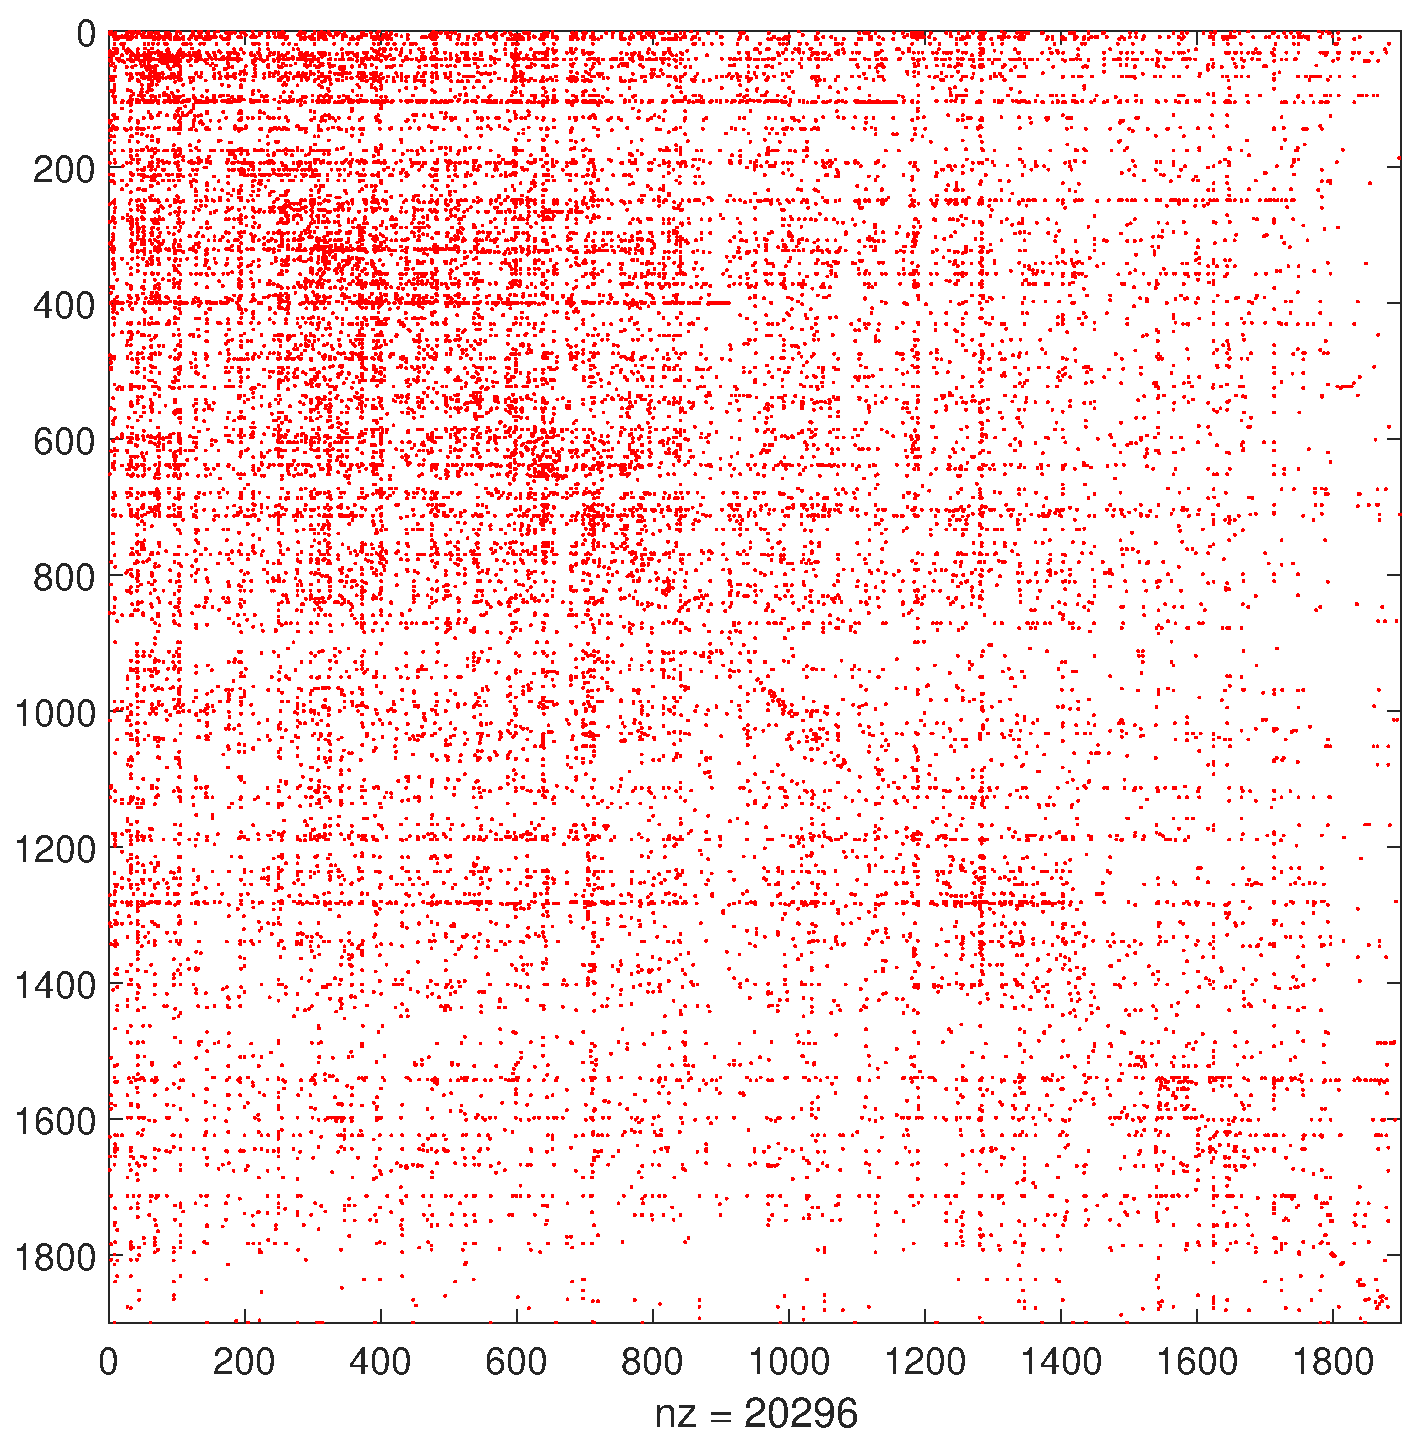
\includegraphics[width=0.7\textwidth, height = 0.7\textwidth]{figures/collage_msg_spy.eps}
        \caption{Σχεδιάγραμμα \code{spy} του μητρώου \textit{\texten{CollegeMsg}}  }
        \label{fig:collage_msg_spy}
    \end{figure} 
    \begin{enumerate}
        \setcounter{enumi}{2}
        \item Απο το παραπάνω διάγραμμα ίσως είναι δύσκολο να γίνει αντιληπτό ότι το μητρώο είναι όντως ένα 
            αραιό μητρώο, λόγο μεγέθους του διαγράμματος. Για τον λόγο αυτό, υπολογίζεται η 
            αραιότητα\footnotemark{} του μητρώου  με μεγέθος $1899 \times 1899$  και με $20296$ μη μηδενικά 
            στοιχεία και προκύπτει πώς είναι $99,4\%$ αραιό.
            \footnotetext{Ορισμός από το βιβλίο του \texten{C.Moler} Ενότητα 2.10}
        \item Η υλοποίηση για τον υπολογισμό του  διανύσματος \prank επισυνάπτεται στο Παράρτημα.
        \item Στον Πίνακα \ref{table:pgrank_top20} παρουσιάζονται οι \texten{"top 20"} κόμβοι όπως μας  
            συζητήθηκε  από την εκφώνηση.
    \end{enumerate}
    \begin{table}[h!]
        \centering
        \begin{tabular}{||c | c||}
            \hline    
            \textbf{κόμβος}     &\textbf{τιμή \texten{PR}}  \tabularnewline\hline
            105     &0.009188                              \tabularnewline\hline
            9       &0.008768                               \tabularnewline\hline
            3       &0.008132                              \tabularnewline\hline
            32      &0.007892                              \tabularnewline\hline
            103     &0.007773                              \tabularnewline\hline
            400     &0.007483                              \tabularnewline\hline
            249     &0.007032                              \tabularnewline\hline
            713     &0.006904                              \tabularnewline\hline
            42      &0.006866                              \tabularnewline\hline
            12      &0.005936                              \tabularnewline\hline
            41      &0.005888                              \tabularnewline\hline
            67      &0.0054601                              \tabularnewline\hline
            638     &0.005408                              \tabularnewline\hline
            194     &0.005373                              \tabularnewline\hline
            1713    &0.005240                              \tabularnewline\hline
            1624    &0.005186                              \tabularnewline\hline
            357     &0.005096                              \tabularnewline\hline
            1281    &0.004641                              \tabularnewline\hline
            1283    &0.004598                              \tabularnewline\hline
            523     &0.004579                              \tabularnewline\hline
        \end{tabular}
        \caption{\texten{Top 20} κόμβοι του μητρώου \textit{\texten{CollegeMsg}} } 
        \label{table:pgrank_top20}
    \end{table}
\newpage    
    \begin{enumerate}
        \setcounter{enumi}{5}
        \item Στο υποερώτημα αυτό υπολογίσαμε τον δείκτη κατάστασης $\kappa_\infty$ του μητρώου $(Ι - pGD)$  για 
            διάφορες τιμές της πιθανότητας $p$ του τυχαίου περιπάτου. Tα αποτελέσματα\footnotemark{}  
            παρουσιάζονται παρακάτω στον Πίνακα \ref{table:cond}. Παρατηρείτε ότι όσο μεγαλώνει η πιθανότητα 
            αυξάνεται αρκετά και ο δείκτης κατάστασης, δηλαδή το μητρώο τείνει να γίνει µη αντιστρέψιµο.
            Καθώς το $p$ πλησιάζει προς το 1, τότε το μητρώο $G$ (μητρώο συνδέσιμοτητας) χάνει την αραιότητά του
            , αφού η πιθανότητα να επιλεγεί ένας τυχαίος συνδεσμος($1-p$) τήνει στο 0,  και προκύπτει η
            αστάθεια στα παραγόμενα αποτελέσματα.
            \footnotetext{Χρησιμοποιηθηκε η συνάρτηση \code{cond} της \matl και σαν είσοδο δώθηκε η  
            \code{full} δομη  των μητρώων $G,D$ }
    \end{enumerate}
    \begin{table}[h!]
        \centering
        \begin{tabular}{c c}
            \hline  
            $\boldsymbol{p}$    &$\boldsymbol{\kappa_\infty}$               \tabularnewline\hline
            0.25            & 128                             \tabularnewline
            0.45            & 445                               \tabularnewline
            0.65            & 1192                              \tabularnewline
            0.85            & 3998                             \tabularnewline
            0.95            & 14212                              \tabularnewline
            0.99            & 75158                              \tabularnewline
            \hline  
        \end{tabular}
        \caption{Δείκτης κατάστασης μητρώου $(Ι - pGD)$ για διαφορές τιμες  $p$ } 
        \label{table:cond}
    \end{table}
\newpage

\begin{center}
    \section*{Παράρτημα} 
    Σε αυτό το σημείο παρατίθενται τα αρχεία \matl  που εκτελέστηκαν για την εξαγωγή των αποτελεσμάτων της 
    εργασίας αυτής. Όλα τα αρχεία βρίσκονται μεσα στο φάκελο \code{".../matlab"} του ζιπαρισμένου αρχείου. 
\end{center}
\subsection*{ \underline{\texten{Matlab script \smw}}}
    \begin{itemize}
        \item[-] 
            \texttt{\texten{MxMake\_1467.m}}
            \texten{\lstinputlisting{matlab/smw/MxMake_1467.m}}
        \item[-] 
            \texttt{\texten{SMW\_solve\_1467.m}}
            \texten{\lstinputlisting{matlab/smw/SMW_solve_1467.m}}     
        \item[-] 
            \texttt{\texten{SMW\_test\_1467.m}}
            \texten{\lstinputlisting{matlab/smw/SMW_test_1467.m}}                 
    \end{itemize}

\subsection*{ \underline{\texten{Matlab script \prank}}}
    \begin{itemize}
        \item[-] 
            \texttt{\texten{PageRank\_1467.m}}
            \texten{\lstinputlisting{matlab/page_rank/PageRank_1467.m}}
    \end{itemize}
\end{document}
